\documentclass{standalone}
\usepackage{pgfplots}
\begin{document}
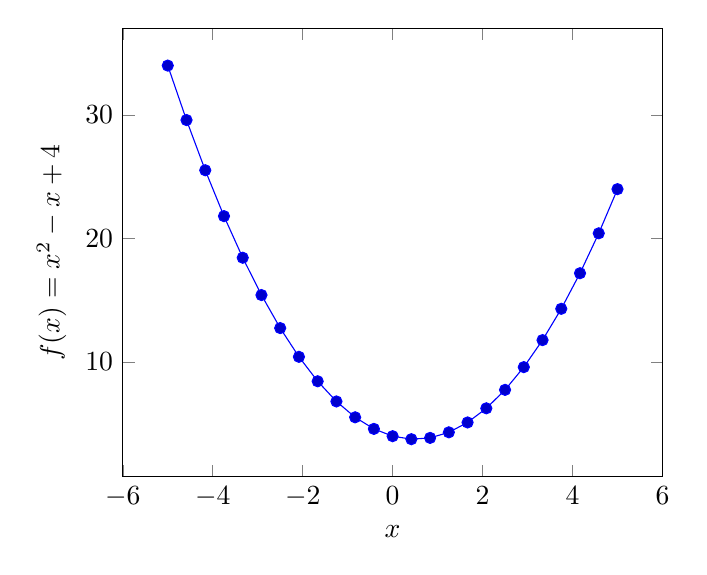
\begin{tikzpicture}
\begin{axis}[
    xlabel=$x$,
    ylabel={$f(x) = x^2 - x +4$}
]
% use TeX as calculator:
\addplot {x^2 - x +4};
\end{axis}
\end{tikzpicture}
\end{document}
